\documentclass[11pt]{article}

% Official ACL style, review mode: anonymous, line numbers. Do not edit acl.sty.
\usepackage[review]{acl}

\usepackage{times}
\usepackage{latexsym}
\usepackage[T1]{fontenc}
\usepackage[utf8]{inputenc}
\usepackage{microtype}
\usepackage{inconsolata}
\usepackage{graphicx}
\usepackage{booktabs}
\usepackage{xcolor}
\usepackage{tfrupee}

% Visible markers for items that need a human decision before submission.
\newcommand{\todo}[1]{\textcolor{red}{\textbf{[TODO:} #1\textbf{]}}}
\newcommand{\rs}{\rupee}
\newcommand{\form}[1]{\textbf{#1}}

\title{Romanized Hindi, Not Code-Mixing: A Controlled Audit of\\ Hinglish Math Evaluation in Small LLMs}

\author{Anonymous}

\begin{document}
\maketitle

\begin{abstract}
We ask whether the language form of an otherwise identical math word problem changes whether a small open LLM solves it. Each problem family is rendered as English (E), Romanized Hindi (R) and Roman-script code-mixed Hinglish (C), with code-computed gold, blind dual-LLM verification and bilingual human review. On 36 permanently excluded fixture prompts, the original answer-format instruction made 10/36 Qwen3-4B outputs fail strict scoring and pushed 8/12 Romanized-Hindi explanations into Devanagari; one disclosed prompt revision reduced both to zero. Format compliance was strongly model-specific across seven models; the remaining errors involved the operation words \emph{bhaag} (divide) and \emph{bhinn} (fraction, also ``different''). On 70 human-reviewed families (210 prompts per model) under a pre-registered plan, Romanized Hindi is the weakest form for all three backbones: Qwen3-4B scores 94.3/85.7/94.3\% on E/R/C, Qwen3-8B 98.6/91.4/98.6\%, and Llama-3.2-3B 94.3/57.1/70.0\%. Code-mixed input is as easy as English for both Qwen models. R errors are not concentrated in items with Hindi operation words, so the misreading hypothesis is not supported.
\end{abstract}

\section{Introduction}

A model that answers ``How many marbles does Aman have?'' may fail on \emph{Aman ke paas kitne kanche hain?} although the mathematics is identical. A drop could come from vocabulary, spelling, mixing, wording or the evaluation protocol itself, so we hold the mathematics fixed and vary only the form.

Lower accuracy on code-mixed or Romanized math input has been reported before \citep{yang-chai-2025-codemixbench,sarvam-2025-sarvamm,sthanika-2026-codemix}, so an E/R/C gap is not new by itself. Our contributions are narrower: (1)~\textbf{a measurement caution}: on excluded fixtures, a plausible final-answer instruction caused form-dependent scoring failures and output-language drift, and format compliance varied widely across seven models; (2)~\textbf{a paired, reviewed E/R/C resource} in which C keeps or switches R's Hindi operation words in balanced proportions; (3)~\textbf{a frozen diagnostic pilot} with strict and numeric endpoints. All development evidence (\S\ref{sec:dev}) comes from 12 fixture families permanently excluded from every split; none of it is a pilot result.

\section{Related Work}

\paragraph{Hindi and multilingual math.} MGSM translates GSM8K \citep{cobbe-etal-2021-gsm8k} into ten languages, but not Hindi \citep{shi-etal-2023-mgsm}. GSM8K-Hi is a human-verified machine translation of GSM8K into Devanagari \citep{kamath-etal-2025-benchmarking}, and HAWP has 2,336 Hindi arithmetic problems \citep{sharma-etal-2022-hawp}. \citet{anand-etal-2025-multilingual} tune on Hindi and English math, excluding Romanized Hindi. mCoT \citep{lai-nissim-2024-mcot}, MathOctopus \citep{chen-etal-2024-breaking} and XCOT \citep{chai-etal-2025-xcot} study multilingual math training.

\paragraph{Code-mixed and Romanized evaluation.} Models score lower on CodeMixBench's Devanagari--Latin Hindi--English GSM8K than on English \citep{yang-chai-2025-codemixbench}. Indi-RomCoM varies Romanized code-mixing intensity \citep[preprint]{das-etal-2026-indiromcom}. An author report aligns GSM8K across five script and register forms, including Romanized Hindi and Hinglish \citep{sthanika-2026-codemix}. The Sarvam-M report shows GSM8K accuracy falling from native-script to Romanized Indic input for every listed model \citep{sarvam-2025-sarvamm}, and a similar penalty appears for health queries \citep[preprint]{khullar-etal-2025-script}. Ours are newly drafted rather than GSM8K-derived, all in Roman script, and human-reviewed.

\paragraph{Operation cues and spelling.} Math solvers exploit shallow cues \citep{patel-etal-2021-nlp}, and LLMs turn irrelevant phrases into operations \citep{mirzadeh-etal-2025-gsmsymbolic}. Romanized Hindi has no standard orthography \citep{bali-etal-2014-borrowing,roark-etal-2020-processing}. Token counts differ across languages \citep{petrov-etal-2023-tokenizers}; we treat them only as correlates. A bounded search found no study isolating Hindi operation-word polysemy as a cause of LLM math errors (a search limit, not a novelty claim).

\section{Data}
\label{sec:data}

\paragraph{Families and forms.} A family is one problem with three renderings. \form{E} is English; \form{R} is Hindi phrasing in Roman script, with a borrowing list for numbers, units and established loanwords; \form{C} is Roman-script Hindi with English lexical material beyond that list. Six topics (comparison, money, fractions/percentages, ratios, rates/units, algebra) are covered; the original pilot has 30 families (five per topic) and Pilot-B adds 70 (12/12/12/12/11/11).

\paragraph{AI drafting, code gold, blind verification.} All families were LLM-drafted, with gold computed in code: Claude (claude-opus-5-5) drafted Pilot-B, and a separate Phase-2 set (100 FINAL\_TEST, 40 DEV, 160 TRAIN) was drafted by GPT for test and development and by Claude for training \todo{GPT model version; drafting model of the original 30}. Claude and GPT each solved every rendering blind in a fresh context; no Qwen model ever drafted, solved or checked. On Pilot-B both solvers matched gold on 210/210 first-version and 15/15 revised renderings. On 900 Phase-2 renderings, Claude matched 900/900 and GPT 897/900 (all misses in one family, gold confirmed by hand). Solver agreement shows only that the text encodes the specified calculation; the solvers may share blind spots.

\paragraph{Bilingual human review.} Each of the original 30 families gets two independent blind solves and an adjudicator \todo{completion status of R01/R02 review and A01 adjudication}. One bilingual team member reviewed all of Pilot-B: 57 ACCEPT, 13 REVISE, 0 REJECT, with two equivalence failures. One bilingual team member \todo{same reviewer as Pilot-B?} also reviewed all of FINAL\_TEST (32 ACCEPT, 68 REVISE). GPT-drafted Romanized Hindi was systematically over-formal: 68/100 GPT-drafted families needed repair, against 13/70 Claude-drafted families. This is descriptive: drafter is confounded with split, prompt and review timing, and the counts are family-level dispositions \todo{share of REVISE decisions that targeted R}. The reviewer also confirmed AI-assistant edits that kept R distinct from C (53 OK, 30 EDIT, 5 MINE) \todo{define EDIT/MINE}. No second annotator has reviewed these families yet.

\paragraph{C as insertional Hinglish.} Review showed natural Hinglish to be mostly \emph{insertional}: Hindi grammar with English nouns, conjunct verbs and relation words (\emph{23 add karta hai}). Pilot-B and Phase~2 C therefore require English material beyond R's borrowing list but no English clause; the original 30 keep the earlier clause-based definition and are reported separately.

\paragraph{Operation-word lexicon and keep/switch balance.} An AI research assistant proposed 25 Hindi operation-word families with spelling variants, flagged as lexically ambiguous (\emph{bhinn} ``fraction''/``different''; \emph{bhaag} ``divide''/``run'') or context-dependent (\emph{kam}). One bilingual team member reviewed all entries (13 of them AI- or dictionary-assisted, then endorsed); \emph{anupat} (ratio) remains unconfirmed. On the original 30 drafts, a fixed matcher finds lexicon words in 27/30 R but only 10/30 C renderings, so a C advantage there could partly reflect easier vocabulary. Pilot-B counters this: C \emph{keeps} R's Hindi operation word in 18 families, \emph{switches} it to English in 17, and 35 are controls without one. FINAL\_TEST and DEV follow the same design (25/25/50; 10/10/20) \todo{first-version drafting tags; recount on accepted text with the frozen matcher}.

\section{Protocol}
\label{sec:protocol}

\paragraph{Prompt and scoring.} One English instruction (\texttt{test1-english-final-v2}) is used for every form. It asks for a short explanation in English and a final line beginning \texttt{FINAL:}, followed by an English unit only when the answer has one and by nothing after a pure number \todo{quote exact prompt text in appendix}. It was revised once on excluded data (\S\ref{sec:dev}), then frozen. The primary endpoint is a frozen strict scorer (v1.0.0): exactly one terminal \texttt{FINAL:} line, an exact rational value, and a unit validated against pre-declared aliases and conversions; missing, refused, ambiguous and truncated answers count as wrong. The secondary endpoint, \texttt{numeric\_literal\_v1}, adopted before the pilot, checks whether the literal value on the sole FINAL line equals gold. It is reported beside, never instead of, the strict endpoint; disagreement does not prove a format-only error. One bilingual auditor tags every output with a fixed error taxonomy and English compliance \todo{auditor/spot-checker assignment for Pilot-B}.

\paragraph{Models.} The primary backbone is Qwen3-4B \citep{qwen3-2025} at revision \texttt{1cfa9a72\ldots}, with NF4 4-bit quantization \citep{dettmers-etal-2023-qlora}, FP16 compute, thinking disabled, greedy decoding, a 1,024-token cap and a fresh context per prompt, on a Colab T4. Qwen3-8B and Llama-3.2-3B-Instruct are secondary, descriptive backbones under the identical protocol. Both passed a rule declared before screening: at most 3/36 strict-invalid fixture outputs under the unchanged prompt and scorer, with no per-model tuning.

\begin{table}[t]
\centering
\small
\setlength{\tabcolsep}{2.6pt}
\begin{tabular}{@{}lrcl@{}}
\toprule
Model & Inv. & E/R/C & Dominant failure \\
\midrule
Qwen3-1.7B$^\times$ & 36 & 0/0/0 & instruction echo \\
Qwen3-4B$^\dagger$ & 0 & 12/10/12 & 2 R op-word misreadings \\
Qwen3-8B & 0 & 12/12/12 & none (1 R in Devanagari) \\
Llama-3.2-3B & 2 & 12/9/9 & value errors in R, C \\
Phi-4-mini$^\times$ & 14 & 6/4/11 & inline FINAL; R repetition \\
Granite-3.3-2B$^\times$ & 36 & 0/0/0 & commentary after FINAL \\
Gemma-3-4B$^\times$ & -- & -- & no outputs (CUDA, FP16) \\
\bottomrule
\end{tabular}
\caption{Format screening on the excluded fixtures (prompt v2; strict-invalid of 36; strict correct of 12 per form). $^\dagger$primary; $^\times$excluded from the pilot. Phi-4-mini and Granite were excluded before the $\le$3/36 rule was formalized; both exceed it.}
\label{tab:screen}
\end{table}

\begin{table}[t]
\centering
\small
\setlength{\tabcolsep}{2.4pt}
\begin{tabular}{@{}lccc@{}}
\toprule
Backbone & E & R & C \\
\midrule
Qwen3-4B & 94.3 {\scriptsize[86.2, 97.8]} & 85.7 {\scriptsize[75.7, 92.1]} & 94.3 {\scriptsize[86.2, 97.8]} \\
\quad invalid & 3 & 2 & 1 \\
Qwen3-8B & 98.6 {\scriptsize[92.3, 99.7]} & 91.4 {\scriptsize[82.5, 96.0]} & 98.6 {\scriptsize[92.3, 99.7]} \\
\quad invalid & 1 & 1 & 0 \\
Llama-3.2-3B & 94.3 {\scriptsize[86.2, 97.8]} & 57.1 {\scriptsize[45.5, 68.1]} & 70.0 {\scriptsize[58.5, 79.5]} \\
\quad invalid & 1 & 6 (5) & 4 (2) \\
\bottomrule
\end{tabular}
\caption{Strict accuracy (\%) by form, Pilot-B, 70 families, with 95\% Wilson intervals. \emph{invalid}: strict-invalid outputs (truncated in parentheses). No refusals occurred. Qwen3-4B is primary.}
\label{tab:acc}
\end{table}

\begin{figure*}[t]
\centering
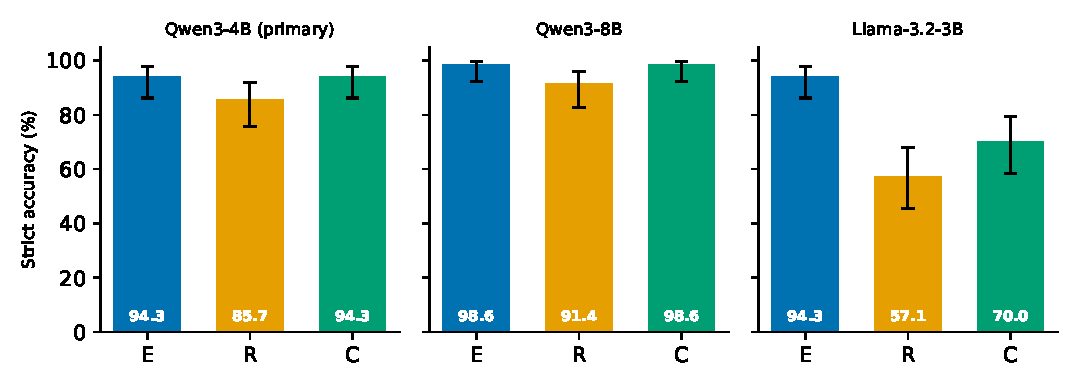
\includegraphics[width=0.62\textwidth]{figures/accuracy_by_form.pdf}
\caption{Strict accuracy by form with 95\% Wilson intervals, Pilot-B (70 families per bar).}
\label{fig:acc}
\end{figure*}

\begin{table*}[t]
\centering
\small
\begin{tabular}{@{}lccc@{}}
\toprule
Backbone & E$-$R & E$-$C & R$-$C \\
\midrule
Qwen3-4B & $+$8.6 [$-$1.4, $+$18.6] (9/3) & 0.0 [$-$7.1, $+$7.1] (3/3) & $-$8.6 [$-$15.7, $-$1.4] (1/7) \\
Qwen3-8B & $+$7.1 [0.0, $+$14.3] (6/1) & 0.0 [$-$4.3, $+$4.3] (1/1) & $-$7.1 [$-$14.3, 0.0] (1/6) \\
Llama-3.2-3B & $+$37.1 [$+$24.3, $+$50.0] (28/2) & $+$24.3 [$+$11.4, $+$37.1] (21/4) & $-$12.9 [$-$27.1, $+$1.4] (10/19) \\
\bottomrule
\end{tabular}
\caption{Paired family differences (percentage points) with 95\% intervals from 10,000 family-bootstrap resamples (seed 101). In parentheses: discordant families correct only in the first / only in the second form.}
\label{tab:diff}
\end{table*}

\section{Development Findings (Not Results)}
\label{sec:dev}

Everything here comes from 36 AI-authored, unreviewed fixture prompts (12 families $\times$ E/R/C) that are \textbf{permanently excluded} from the pilot and all later data. With 12 prompts per form, every rate is only an indication.

\paragraph{Format confound and v1$\to$v2.} Under the original instruction (\texttt{FINAL: <number or fraction> <unit when applicable>}), 10/36 Qwen3-4B outputs were strict-invalid, all \texttt{invalid\_unit}; strict-correct counts were 9/7/9 on E/R/C. In 8, a unit word was appended to a dimensionless answer (\texttt{8 unitless}), roughly equally across forms; in one R output a Hindi noun became the unit (\texttt{109 moti}). With v2 there were 0/36 invalid outputs, strict and numeric endpoints agreed on all 36, and strict-correct counts were 12/10/12. The fixtures also changed between runs (one R rendering repaired, one alias added), so 10$\to$0 is a development comparison, not an isolated prompt effect. \textbf{Devanagari drift:} under v1, 8/12 R explanations contained Devanagari despite the English instruction (0/12 for E and for C); under v2, 0/12. The detector is heuristic.


\paragraph{Cross-model format compliance.} Six more models ran on the same prompts under frozen v2 (Table~\ref{tab:screen}). Phi-4-mini's inline FINAL lines (rejected by both endpoints) and R repetition to the token cap (6/12) make its C\,>\,E ordering a formatting artifact; Gemma-3-4B's CUDA error is possibly overflow (unconfirmed). Within Qwen3, instruction following broke before mathematics did (36/36 invalid at 1.7B, 0/36 at 4B and 8B). Without a compliance check on excluded data, a multi-model comparison would mostly measure formatting.

\paragraph{Repeated \emph{bhaag}/\emph{bhinn} misreadings.} Under v2, Qwen3-4B's only errors were two R items whose renderings an AI assistant, not an independent bilingual check, judged correct \todo{confirm}. \emph{Bhaag dekar bhinn likho} (``divide, write as a fraction'') was answered as a difference, and \emph{kitna bhinn istemaal hua} (``what fraction was used'') received the remaining count (20) under both v1 and v2. Llama-3.2-3B gave the same 20, so this misreading recurs in a second model family; \emph{Bhinn} means both ``fraction'' and ``different'' even in Devanagari, so the ambiguity is lexical. With $n=2$ unreviewed items, these errors are \emph{consistent with} operation-word misreading but do not establish it. They motivated the lexicon and keep/switch design, fixed before any pilot output.

\section{Pilot Results}
\label{sec:results}

We report the Pilot-B cohort (70 families, single bilingual reviewer; \S\ref{sec:data}), analysed under a pre-registration committed before any Pilot-B output. Each backbone ran once and completed 210/210 renderings; tables reproduce exactly from stored scores. The original 30-family pilot, under two-reviewer adjudication, will be reported separately \todo{R01/R02/A01 status} and is never pooled with Pilot-B.




\paragraph{Romanized Hindi is the hard case.} R is the lowest-scoring form for every backbone (Tables~\ref{tab:acc} and~\ref{tab:diff}, Figure~\ref{fig:acc}). The deficit is modest for Qwen (8.6 and 7.1 points; intervals touch zero) and large for Llama (37.1 points, [$+$24.3, $+$50.0]). Moving from Qwen3-4B to 8B improves all forms but leaves the R deficit roughly unchanged.

\paragraph{Code-mixing is not the problem.} For both Qwen models C matches E exactly (E$-$C $=$ 0.0) and exceeds R; for Qwen3-4B the R$-$C interval excludes zero. For Llama, C lies between E and R. Mixing in English lexical material does not hurt and appears to help relative to Romanized Hindi alone.

\paragraph{The operation-word hypothesis is not supported.} In a pre-registered descriptive split by whether C keeps or switches R's Hindi operation word (or R has none), R accuracy is similar across strata for every model (keep/switch/none): Qwen3-4B 89/82/86\%, Qwen3-8B 94/94/89\%, Llama 67/59/51\%. The R deficit is therefore not concentrated in items with \emph{bhaag}/\emph{bhinn}-type vocabulary. Many Llama R errors are arithmetic slips on simple items (e.g., $1200 - 3\times265$ answered as 435).

\paragraph{Residual format effects.} The secondary numeric endpoint agrees with strict scoring on every Llama rendering, so its gaps are not formatting artifacts. For Qwen, the pre-registered secondary grammar does not accept a \emph{trailing} rupee symbol (\texttt{FINAL: 1575 \rs}), which strict scoring accepts; this accounts for every strict-correct/numeric-fail case (30 for Qwen3-4B, 36 for Qwen3-8B). We report the secondary endpoint as specified; a post-hoc allowance for the trailing symbol restores agreement. Three of Qwen3-4B's four E failures are numerically correct answers with unlisted English unit phrases (\texttt{11 years old}, \texttt{4 bags of cement}), and one C failure is an unlisted spelling (\texttt{300 rupye}): the form-dependent alias penalty anticipated in \S\ref{sec:dev}.

\paragraph{Exploratory (not pre-registered).} Despite the English-explanation instruction, Llama explained 60/70 R and 27/70 C outputs in Romanized-Hindi prose (heuristic detection). On C, Hindi-prose explanations were correct 13/27 against 36/43 for English explanations. This association is confounded by item difficulty and awaits the planned English-compliance audit \todo{audit results (planned Table 5), from the verified audit sidecar}.

\section{Conclusion}

Holding the mathematics fixed, small open models lose accuracy on Romanized Hindi rather than on code-mixing, by a strongly model-specific amount; answer formats must first be checked on excluded data.

\section*{Limitations}

\begin{itemize}\setlength{\itemsep}{1pt}\setlength{\parskip}{0pt}
\item \textbf{Diagnostic scale.} With at most 100 families per backbone, the vocabulary strata are sparse and descriptive.
\item \textbf{Thin development evidence.} \S\ref{sec:dev} rests on 12 unreviewed fixture families, and the prompt was revised after seeing their outputs; no pilot item was used to design the prompt.
\item \textbf{Single reviewer.} Pilot-B, FINAL\_TEST and the lexicon each had one bilingual reviewer, who is a team member. Part of the lexicon was AI-assisted, and \emph{anupat} is unconfirmed. Naturalness judgments reflect one speaker's register.
\item \textbf{AI-authored data.} Items share LLM drafting styles. Claude both drafted and solved Pilot-B. The GPT/Claude repair contrast is confounded with split and prompt.
\item \textbf{Different C definitions.} The original 30 and Pilot-B define C differently, which prevents a simple pooled C estimate.
\item \textbf{Models.} All backbones are small, quantized, greedy and non-thinking. Admitting models by format compliance excludes families whose formatting the scorer does not accept.
\item \textbf{No script control.} There is no Devanagari arm, so an E--R gap mixes script, language, register and spelling. C $\approx$ E with R $<$ E would suggest vocabulary but would not identify it. Each R rendering is one of many possible spellings.
\item \textbf{Contamination.} The items are new, but the models' pretraining data cannot be audited.
\end{itemize}

\section*{Ethics Statement}

\textbf{Consent and credit.} Reviewers received a consent note covering the task, data use and release \todo{signed consent and exposure records for every reviewer; roles (team member or external); any compensation}. Reviewers will be credited in the camera-ready acknowledgments or as authors, as appropriate and according to their stated preference \todo{confirm each reviewer's preference}. Real identities stay out of shared ledgers.

\textbf{AI-assistance disclosure.} (1) \emph{AI-drafted items:} every rendering was drafted by an LLM (Claude for Pilot-B and the training split, GPT for test and development \todo{drafting model of the original 30}). The families were then checked against code-computed gold, verified blind by two LLM solvers and reviewed by humans. (2) \emph{AI-assisted human review:} humans made every acceptance decision, but some lexicon entries and some text edits were drafted by AI before reviewers confirmed them (\S\ref{sec:data}). (3) \emph{Writing and coding:} AI assistants helped write the evaluation and analysis code, the research notes and this manuscript, and recorded protocol decisions under the authors' delegation. The authors reviewed all of this and take responsibility for it \todo{name the assistant systems per venue policy}.

\textbf{Data.} The items are invented everyday word problems and are not expected to contain personal information \todo{names/PII check before release}. Romanized Hindi varies by region and register, and our renderings reflect few speakers. Data are released under CC BY 4.0 and code under MIT. FINAL\_TEST stays unreleased until the confirmatory evaluation.

\bibliography{references}

\end{document}
